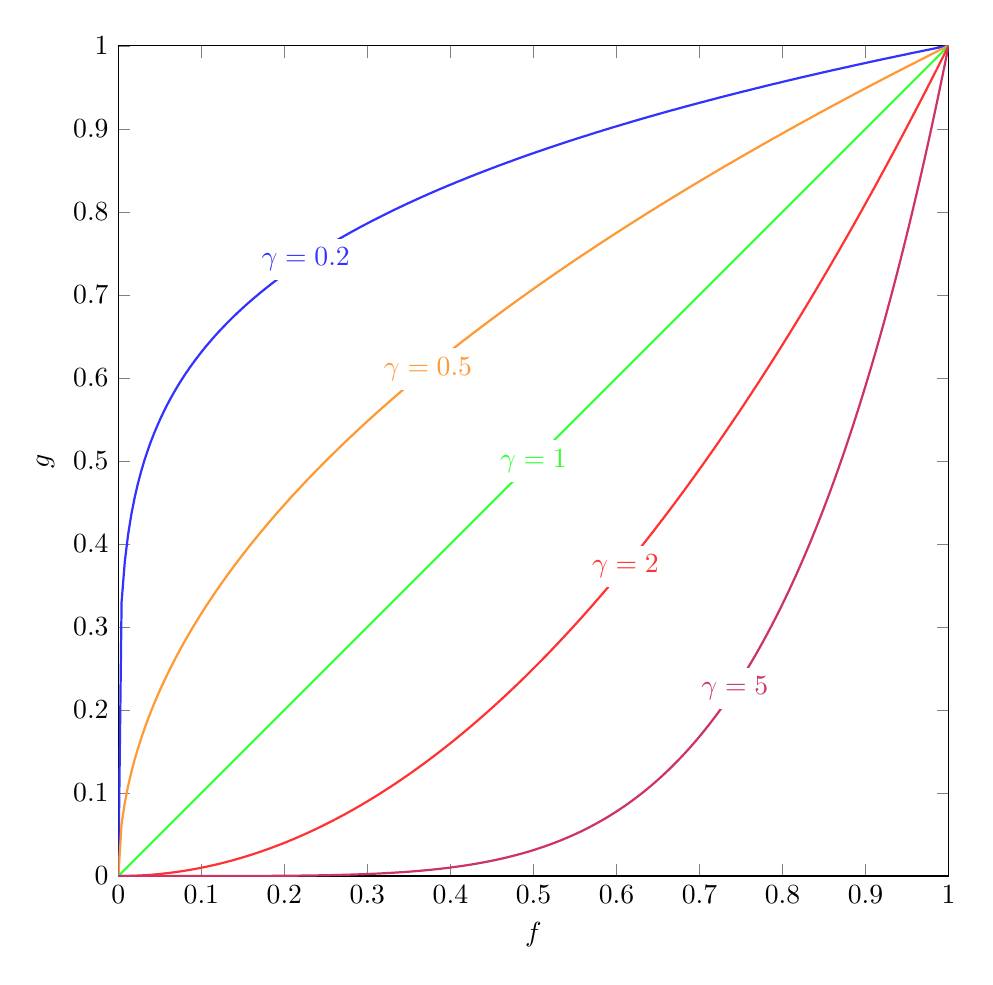
\begin{tikzpicture}
	\begin{axis}
	[
		xmin  = 0,
		xmax = 1,
		ymin = 0,
		ymax = 1,
		%enlarge limits=false,
		axis equal,
		xlabel = {$f$},
		ylabel = {$g$},		
    	legend style={at={(1.2,1)}, anchor=north,legend columns=1},	
		width=\textwidth,
		height=\textwidth    	
	]
	\addplot [domain = 0:1, samples=256, blue!80, thick]  {x^0.2} node[pos=0.5, fill=white] {$\gamma = 0.2$};
	\addplot [domain = 0:1, samples=256, orange!80, thick]  {x^0.5} node[pos=0.5, fill=white] {$\gamma = 0.5$};	
	\addplot [domain = 0:1, samples=256, green!80, thick]  {x^1} node[pos=0.5, fill=white] {$\gamma = 1$};
	\addplot [domain = 0:1, samples=256, red!80, thick]  {x^2} node[pos=0.5, fill=white] {$\gamma = 2$};
	\addplot [domain = 0:1, samples=256, purple!80, thick]  {x^5} node[pos=0.5, fill=white] {$\gamma = 5$};
	%\legend{$\gamma = 0.3$, $\gamma = 0.5$, $\gamma = 1$, $\gamma = 2$, $\gamma = 5$}	
	\end{axis}

\end{tikzpicture} 